\documentclass[a4paper, 12pt]{article}

\usepackage[utf8]{inputenc}
\usepackage{graphicx}
\usepackage{import}
\usepackage{tikz}
\usetikzlibrary{automata}
\usepackage[absolute,overlay]{textpos}
\usepackage{listings}
\usepackage{booktabs} 
\usepackage{rotating}
\usepackage{graphicx}
\usepackage{pdfpages}
\usepackage{longtable}
\usepackage[stable]{footmisc}
\usepackage[a4paper,bindingoffset=0.2in,%
            left=1in,right=1in,top=1in,bottom=1in,%
            footskip=.25in]{geometry}
            
\usepackage{color}
\definecolor{lightgray}{rgb}{.9,.9,.9}
\definecolor{darkgray}{rgb}{.4,.4,.4}
\definecolor{purple}{rgb}{0.65, 0.12, 0.82}

\lstdefinelanguage{JavaScript}{
  keywords={typeof, new, true, false, catch, function, return, null, catch, switch, var, if, in, while, do, else, case, break},
  keywordstyle=\color{blue}\bfseries,
  ndkeywords={class, export, boolean, throw, implements, import, this},
  ndkeywordstyle=\color{darkgray}\bfseries,
  identifierstyle=\color{black},
  sensitive=false,
  comment=[l]{//},
  morecomment=[s]{/*}{*/},
  commentstyle=\color{purple}\ttfamily,
  stringstyle=\color{red}\ttfamily,
  morestring=[b]',
  morestring=[b]"
}    
        
\lstdefinestyle{JavaScript}{
	language=JavaScript,
   backgroundcolor=\color{lightgray},
   extendedchars=true,
   basicstyle=\footnotesize\ttfamily,
   showstringspaces=false,
   showspaces=false,
   numbers=left,
   numberstyle=\footnotesize,
   numbersep=9pt,
   tabsize=2,
   breaklines=true,
   showtabs=false,
   captionpos=b
}      

\lstdefinestyle{DOS}
{
    backgroundcolor=\color{black},
    basicstyle=\scriptsize\color{white}\ttfamily
}


\lstdefinestyle{Gramatica}{
  basicstyle=\itshape\small,
  tabsize=4,
  literate={->}{$\rightarrow$}{2}
           {λ}{$\lambda$}{1}
}

\lstdefinestyle{EstadosAutomataST}{
  basicstyle=\mdseries\footnotesize,
  xleftmargin=0em,
  mathescape=true,
  tabsize=4,
  literate={->}{$\rightarrow$}{2}
           {λ}{$\lambda$}{1}
           {.}{$\bullet$}1
}     

\lstdefinestyle{AccionesSemanticas}{
  basicstyle=\mdseries\small,
  xleftmargin=0em,
  mathescape=true,
  tabsize=4,
}
         
\title{Memoria de la Práctica de Procesadores de Lenguajes}
\author{Diego José Abengózar Vilar, Alejandro García Castellanos,\\ Ignacio Javier Encinas Ramos\\\\Grupo 82}

\renewcommand*\contentsname{Índice}

\begin{document}
\maketitle
\tableofcontents
\newpage
\import{Lexico/}{MemoriaLexicoG82.tex}
\newpage
\import{Sintactico/}{MemoriaSintacticoG82.tex}
\newpage
\section{Anexo de Pruebas Semántico}
\subsection*{Error 1:}
\lstinputlisting[style=JavaScript]{Pruebas/Error1LEX.txt}
\lstinputlisting[style=DOS]{Pruebas/MsgErr1LEX.txt}

\subsection*{Error 2:}
\lstinputlisting[style=JavaScript]{Pruebas/Error2LEX.txt}
\lstinputlisting[style=DOS]{Pruebas/MsgErr2LEX.txt}

\subsection*{Error 3:}
\lstinputlisting[style=JavaScript]{Pruebas/Error3LEX.txt}
\lstinputlisting[style=DOS]{Pruebas/MsgErr3LEX.txt}

\subsection*{Prueba 1 Correcta:}
\lstinputlisting[style=JavaScript]{Pruebas/Prueba1LEX.txt}
\subsubsection*{Tokens:}
\lstinputlisting{Pruebas/Prueba1Tokens.txt}
\subsubsection*{Tabla de símbolos:}
\lstinputlisting{Pruebas/Prueba1TS.txt}

\subsection*{Prueba 2 Correcta:}
\lstinputlisting[style=JavaScript]{Pruebas/Prueba2LEX.txt}
\subsubsection*{Tokens:}
\lstinputlisting{Pruebas/Prueba2Tokens.txt}
\subsubsection*{Tabla de símbolos:}
\lstinputlisting{Pruebas/Prueba2TS.txt}

\subsection*{Prueba 3 Correcta:}
\lstinputlisting[style=JavaScript]{Pruebas/Prueba3LEX.txt}
\subsubsection*{Tokens:}
\lstinputlisting{Pruebas/Prueba3Tokens.txt}
\subsubsection*{Tabla de símbolos:}
\lstinputlisting{Pruebas/Prueba3TS.txt}

\newpage
\section{Anexo de Pruebas Sintáctico}
\subsection*{Error 1:}
\lstinputlisting[style=JavaScript]{Pruebas/Error1ST.txt}
\lstinputlisting[style=DOS]{Pruebas/MsgErr1ST.txt}

\subsection*{Error 2:}
\lstinputlisting[style=JavaScript]{Pruebas/Error2ST.txt}
\lstinputlisting[style=DOS]{Pruebas/MsgErr2ST.txt}

\subsection*{Error 3:}
\lstinputlisting[style=JavaScript]{Pruebas/Error3ST.txt}
\lstinputlisting[style=DOS]{Pruebas/MsgErr3ST.txt}

\subsection*{Prueba 1 Correcta:}
\lstinputlisting[style=JavaScript]{Pruebas/Prueba1ST.txt}
\subsubsection*{Parse a Derechas:}
\input{Pruebas/Prueba1Parse.txt}
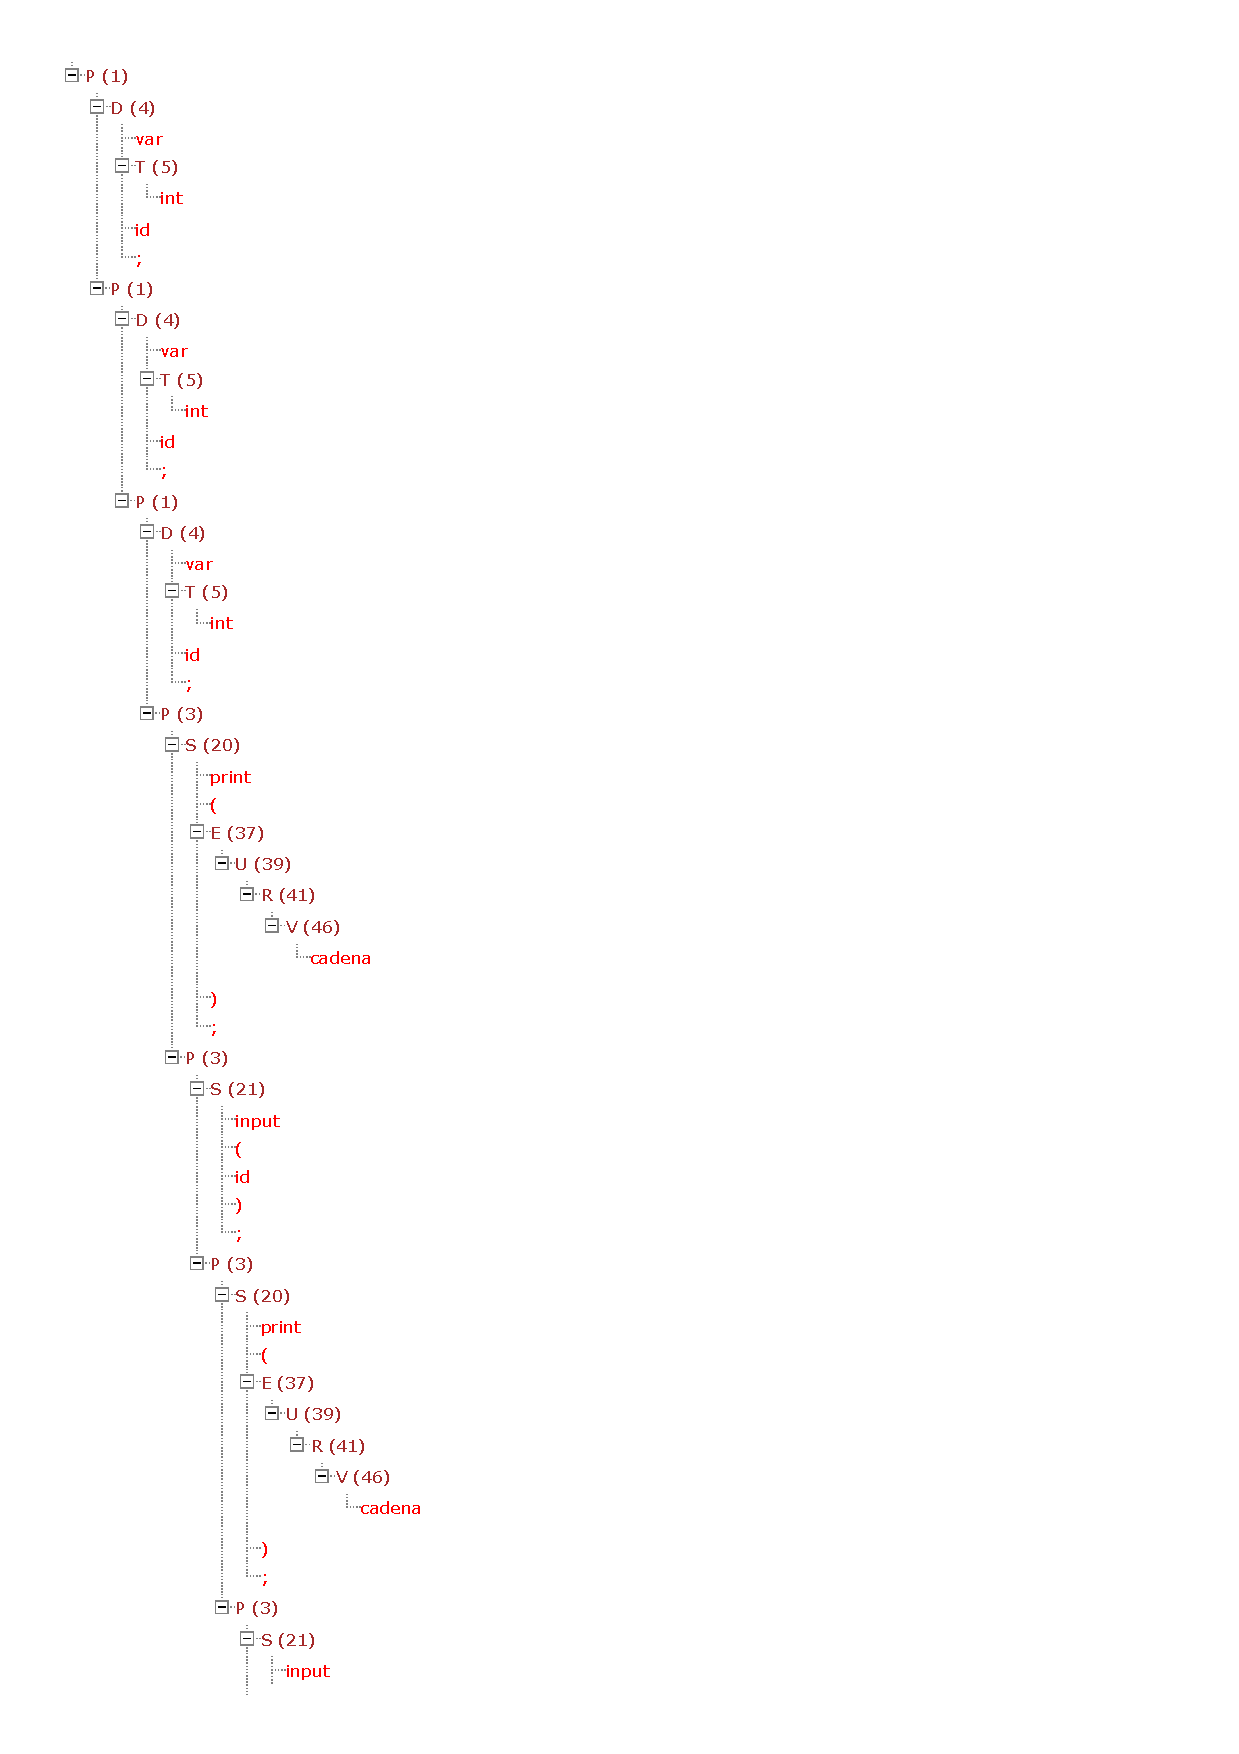
\includepdf[pages=1,pagecommand={\subsubsection*{Árbol sintáctico:}},width=\textwidth]{Pruebas/Prueba1Arbol.pdf}
\includepdf[pages=2-,pagecommand={},width=\textwidth]{Pruebas/Prueba1Arbol.pdf}

\subsection*{Prueba 2 Correcta:}
\lstinputlisting[style=JavaScript]{Pruebas/Prueba2ST.txt}
\subsubsection*{Parse a Derechas:}
\input{Pruebas/Prueba2Parse.txt}
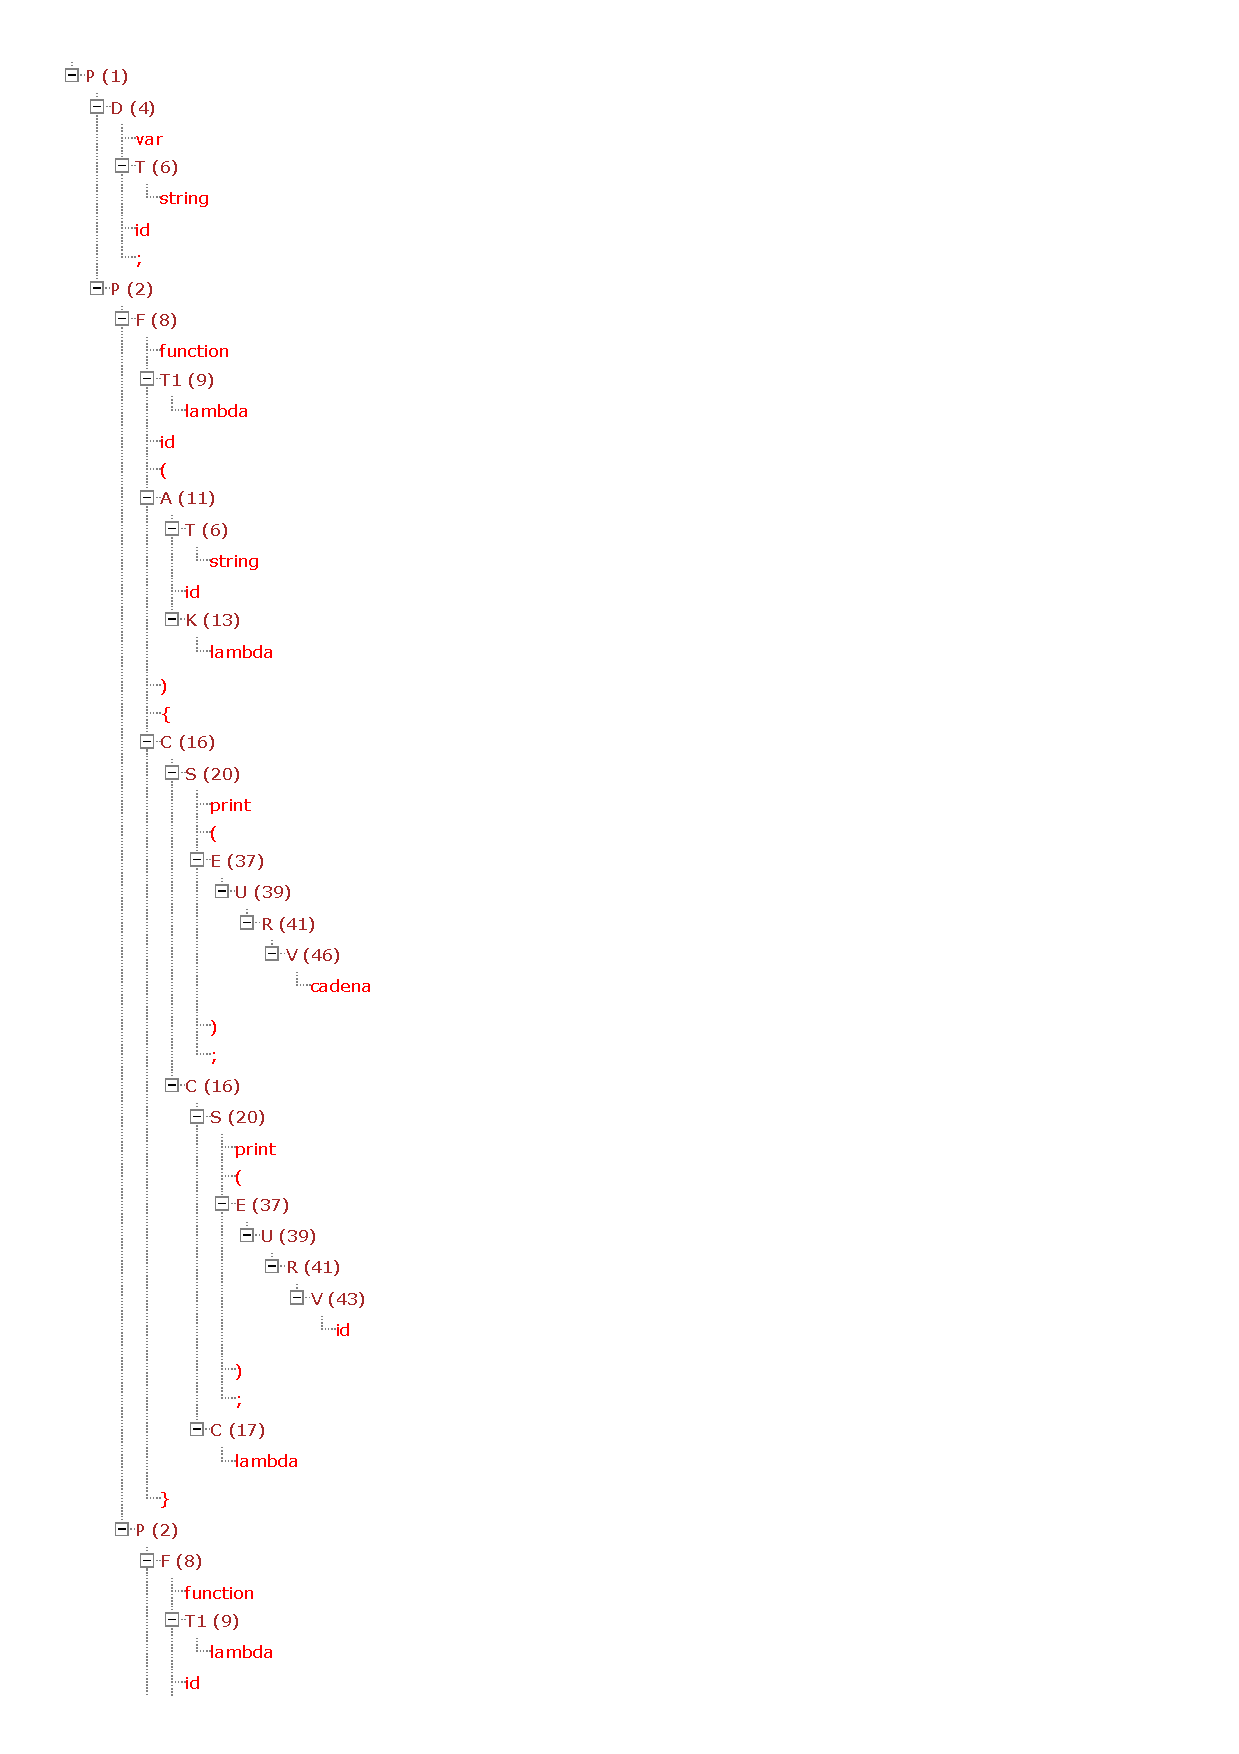
\includepdf[pages=1,pagecommand={\subsubsection*{Árbol sintáctico:}},width=\textwidth]{Pruebas/Prueba2Arbol.pdf}
\includepdf[pages=2-,pagecommand={},width=\textwidth]{Pruebas/Prueba2Arbol.pdf}


\subsection*{Prueba 3 Correcta:}
\lstinputlisting[style=JavaScript]{Pruebas/Prueba3ST.txt}
\subsubsection*{Parse a Derechas:}
\input{Pruebas/Prueba3Parse.txt}
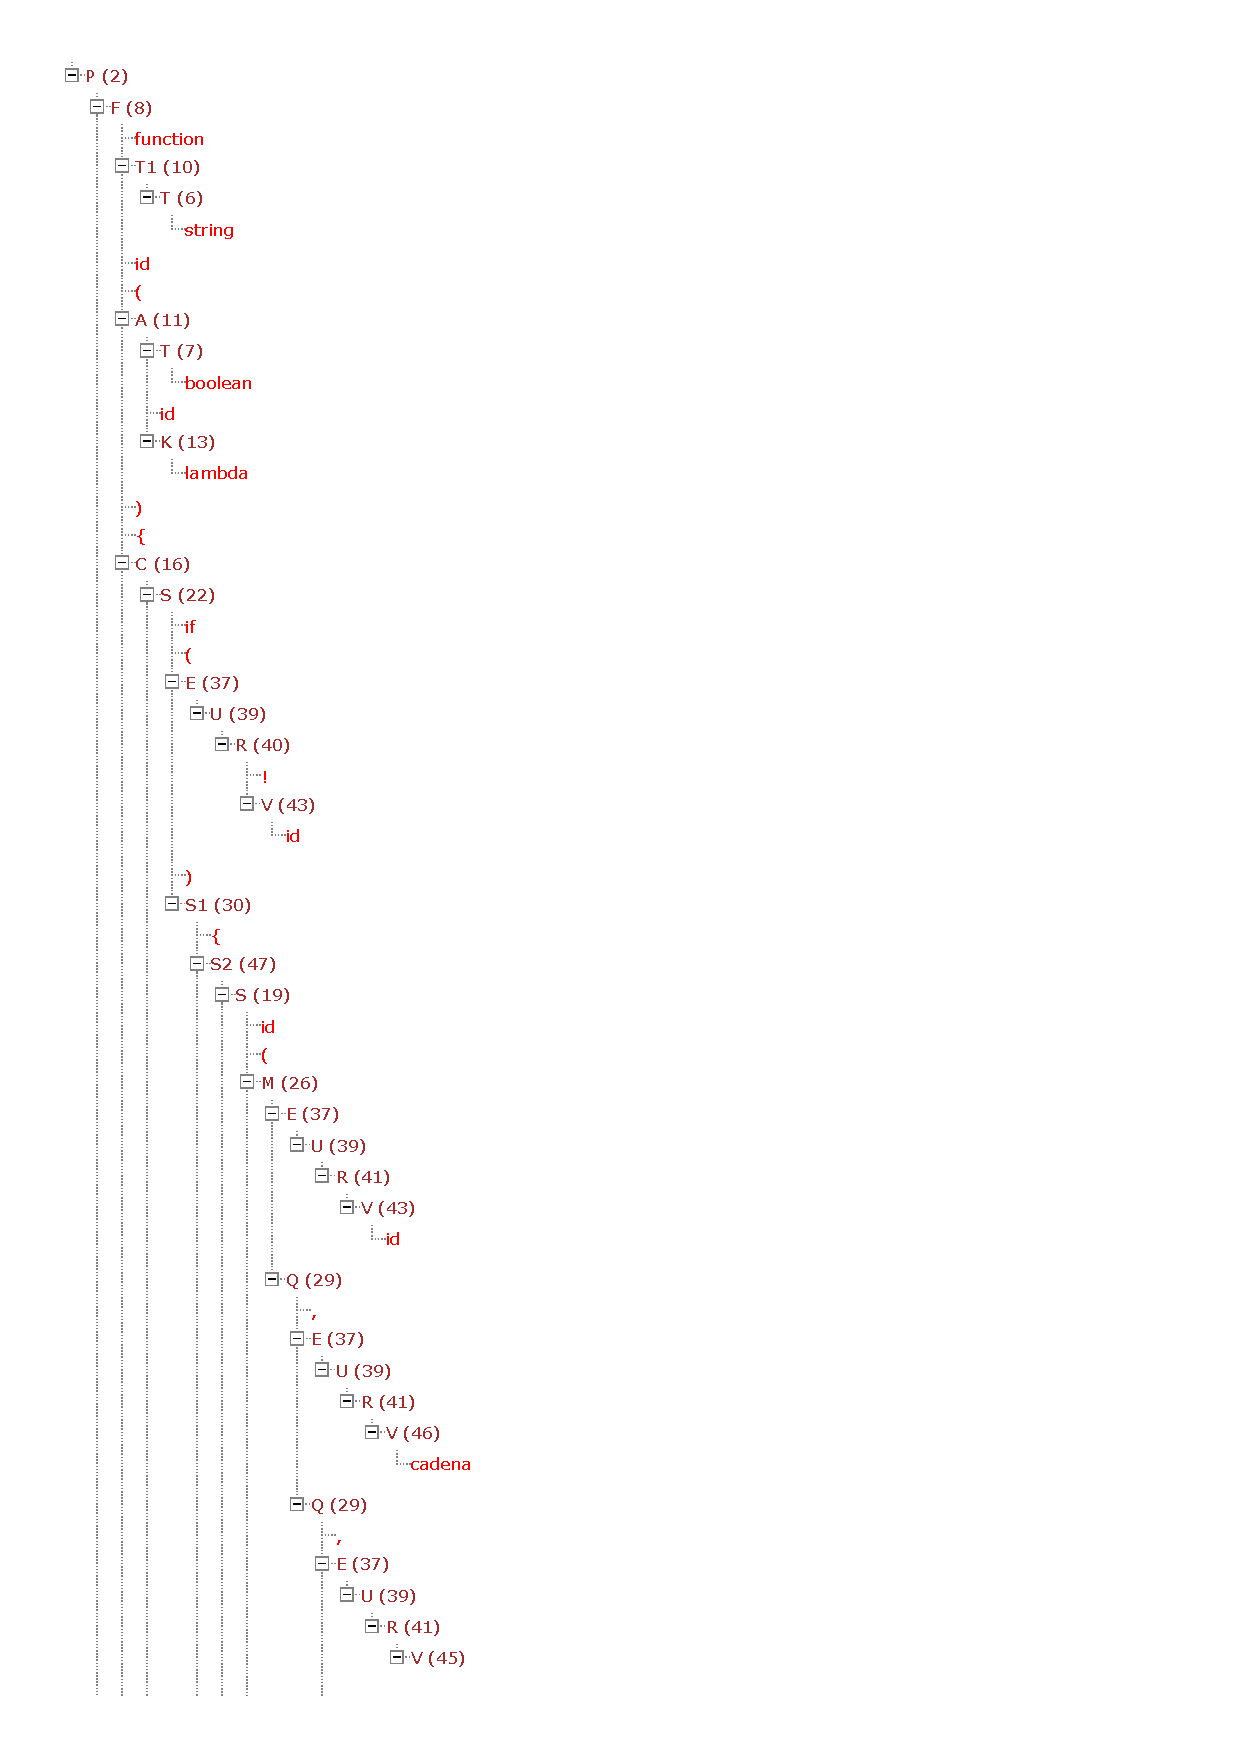
\includepdf[pages=1,pagecommand={\subsubsection*{Árbol sintáctico:}},width=\textwidth]{Pruebas/Prueba3Arbol.pdf}
\includepdf[pages=2-,pagecommand={},width=\textwidth]{Pruebas/Prueba3Arbol.pdf}


\end{document}
